\documentclass[tikz,border=8pt]{standalone}
\usepackage{tikz}
\usepackage{amsmath,amssymb}
\usetikzlibrary{arrows.meta,positioning,calc}

\begin{document}
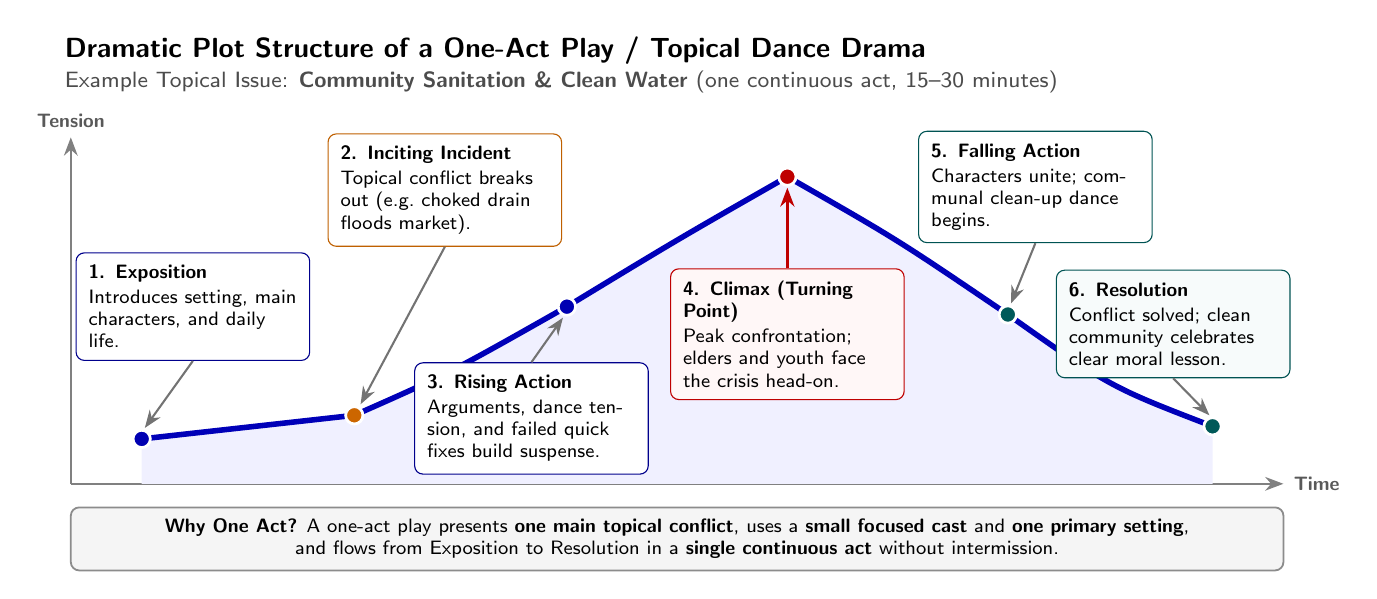
\begin{tikzpicture}[
    font=\sffamily,
    >=Stealth,
    stagebox/.style={
        draw=black!60,
        rounded corners=3pt,
        fill=white,
        text width=2.65cm,
        align=left,
        inner sep=4.5pt,
        font=\sffamily\scriptsize
    }
]

% Title
\node[font=\sffamily\bfseries\normalsize, anchor=west] at (0, 6.65)
    {Dramatic Plot Structure of a One-Act Play / Topical Dance Drama};
\node[font=\sffamily\footnotesize, text=black!70, anchor=west] at (0, 6.25)
    {Example Topical Issue: \textbf{Community Sanitation \& Clean Water} (one continuous act, 15--30 minutes)};

% Baseline / tension axis
\draw[->, line width=0.8pt, black!50] (0.2, 1.15) -- (15.6, 1.15) node[right, font=\sffamily\scriptsize\bfseries, text=black!65] {Time};
\draw[->, line width=0.8pt, black!50] (0.2, 1.15) -- (0.2, 5.55) node[above, font=\sffamily\scriptsize\bfseries, text=black!65] {Tension};

% Plot curve coordinates
\coordinate (P1) at (1.1, 1.72);   % Exposition
\coordinate (P2) at (3.8, 2.02);   % Inciting Incident
\coordinate (P3) at (6.5, 3.40);   % Rising Action
\coordinate (P4) at (9.3, 5.05);   % Climax
\coordinate (P5) at (12.1, 3.30);  % Falling Action
\coordinate (P6) at (14.7, 1.88);  % Resolution

% Shaded area under curve
\fill[blue!6] (1.1, 1.15) -- (P1) -- (P2) .. controls (5.0, 2.55) .. (P3)
    .. controls (7.9, 4.25) .. (P4)
    .. controls (10.7, 4.25) .. (P5)
    .. controls (13.4, 2.38) .. (P6) -- (14.7, 1.15) -- cycle;

% Main plot arc
\draw[line width=2.0pt, blue!72!black]
    (P1) -- (P2)
    .. controls (5.0, 2.55) .. (P3)
    .. controls (7.9, 4.25) .. (P4)
    .. controls (10.7, 4.25) .. (P5)
    .. controls (13.4, 2.38) .. (P6);

% Node markers
\foreach \p/\col in {P1/blue!70!black, P2/orange!80!black, P3/blue!70!black, P4/red!75!black, P5/teal!70!black, P6/teal!70!black} {
    \fill[\col] (\p) circle (0.11);
    \draw[white, line width=1pt] (\p) circle (0.11);
}

% Callout boxes — cleanly separated with generous margins, zero touches!
\node[stagebox, draw=blue!55!black] (B1) at (1.75, 3.40)
    {\textbf{1. Exposition}\\[1pt]Introduces setting, main characters, and daily life.};
\draw[->, black!55, line width=0.75pt] (B1.south) -- ($(P1)+(0.04,0.14)$);

\node[stagebox, draw=orange!75!black] (B2) at (4.95, 4.88)
    {\textbf{2. Inciting Incident}\\[1pt]Topical conflict breaks out (e.g.\ choked drain floods market).};
\draw[->, black!55, line width=0.75pt] (B2.south) -- ($(P2)+(0.08,0.14)$);

\node[stagebox, draw=blue!55!black] (B3) at (6.05, 1.98)
    {\textbf{3. Rising Action}\\[1pt]Arguments, dance tension, and failed quick fixes build suspense.};
\draw[->, black!55, line width=0.75pt] (B3.north) -- ($(P3)-(0.05,0.14)$);

\node[stagebox, draw=red!75!black, fill=red!3] (B4) at (9.30, 3.05)
    {\textbf{4. Climax (Turning Point)}\\[1pt]Peak confrontation; elders and youth face the crisis head-on.};
\draw[->, red!75!black, line width=0.85pt] (B4.north) -- ($(P4)-(0,0.14)$);

\node[stagebox, draw=teal!65!black] (B5) at (12.45, 4.92)
    {\textbf{5. Falling Action}\\[1pt]Characters unite; communal clean-up dance begins.};
\draw[->, black!55, line width=0.75pt] (B5.south) -- ($(P5)+(0.04,0.14)$);

\node[stagebox, draw=teal!65!black, fill=teal!3] (B6) at (14.20, 3.18)
    {\textbf{6. Resolution}\\[1pt]Conflict solved; clean community celebrates clear moral lesson.};
\draw[->, black!55, line width=0.75pt] (B6.south) -- ($(P6)+(-0.04,0.14)$);

% Bottom summary bar
\draw[rounded corners=3pt, draw=black!45, fill=black!4, line width=0.65pt] (0.2, 0.05) rectangle (15.6, 0.85);
\node[font=\sffamily\scriptsize, align=center] at (7.9, 0.45)
    {\textbf{Why One Act?} A one-act play presents \textbf{one main topical conflict}, uses a \textbf{small focused cast} and \textbf{one primary setting},\\and flows from Exposition to Resolution in a \textbf{single continuous act} without intermission.};

\end{tikzpicture}
\end{document}
